\chapter{Introduction and state of the art}\label{Chap1}

\clearpage
\section{Upwelling systems}\label{Chap1UpweSyst}

Oceanography as a science dates back to the late $19^{th}$ century \citep{Wust1964,Mill2012,LlopCowe2014} and studies the oceans and everything related to them, from physical processes to biological ones, that make it a multidisciplinary science. One of the most important physical processes is upwelling whose study interest dates back to the beginning of the $20^{th}$ century \citep{Ogil1912,Murp1920}. Upwelling zones are sites where a fertilization process regularly occurs due to the upward movement of water mass parcels in the water column and to be efficient this process should maintain long enough, at least a few days, in order to upwell deep nutrient-rich water parcels to the surface over a vertical distance of sometimes 100 $m$ or more \citep{Marg1978}.\\

These systems are critical for marine ecosystems and have significant implications for climate and weather patterns since climate should be particularly sensitive to hydrological processes, especially in the tropics \citep{Webs1994}. There are several key upwelling systems around the world, and they typically occur along the western coastlines of continents. The primary form of upwelling is wind-driven upwelling (Fig. \ref{Chap1CoastalUpwelling}). This concept is useful for understanding the coastal ocean's response to wind, as the surface layer of water is moved offshore by the wind and replaced by deeper water upwelling from depth near the coast \citep{BrinHalp1983}. Other forms of upwelling, such as Ekman pumping or equatorial upwelling, will not be discussed here.\\

Since the seawater is a practically incompressible fluid, when there is a vertical upward flow then an equivalent volume of water per unit of time must be displaced in the horizontal direction, when upwelling occurs along the coast with landmass as a boundary, the horizontal displacement is necessarily directed offshore \citep{KampCap2}. Wind-driven coastal upwelling is an efficient way of transporting nutrients from deep to shallow (euphotic) zones in the water column \citep{MessChav2015,MessChav2017} but it is also a source of environmental stress due to widely changing conditions in temperature \citep{CastWang2014}, dissolved oxygen \citep{Scul2010}, and salinity \citep{XuanHuan2012}.\\

The consequence of the upwelling process is the fertilization of the photic zone (Fig. \ref{Chap1UpwellingFertilization}), with waters coming from the deep supplying nutrients such as nitrogen (\textit{N}), phosphorous (\textit{P}), silica (\textit{Si}) and iron (\textit{Fe}, an element that is often limiting) to the surface \citep{GeidLaro1994,BehrBale1996,BehrKolb1999,HutcSedw2001,HutcHare2002,MoorMils2013,HutcBoyd2016,BrisMohr2017}, although nutrient supply may also come from other sources such as river discharge \citep{SharMidd2017} or from the atmosphere \citep{PoweBake2015}.\\

\begin{figure}[H]
	\centering
	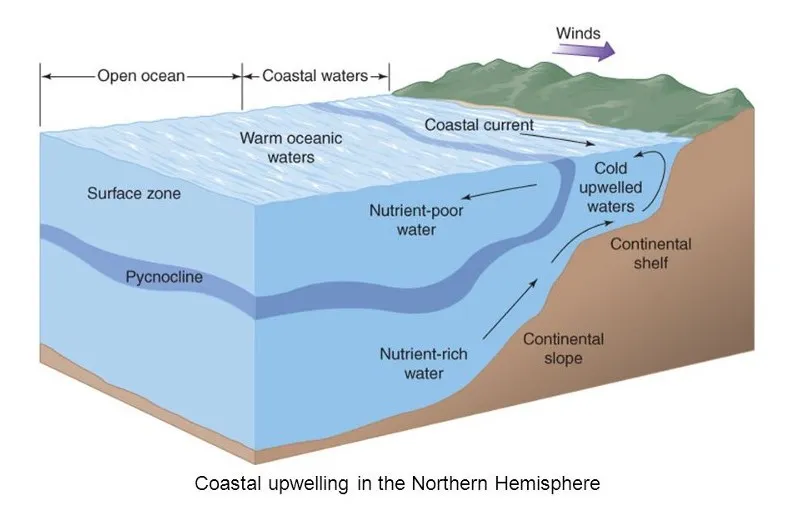
\includegraphics[width=1.0\textwidth]{figures/Chap1CoastalUpwelling.png}
	\caption{Conceptual model of wind-driven upwelling process in the northern hemisphere. It should be noted that in the southern hemisphere, the wind direction is reversed but generates the same upwelling effect.}
	\label{Chap1CoastalUpwelling}
\end{figure}

The process of upwelling can be measured using an index ($upwelling index = \mu \left ( cos\theta -\tau  \right )$) presented by \cite{FielDavi1989}, where $\mu$ represents the wind speed ($ms^{-1}$), $\theta$ represents the wind direction in degrees, and $\tau$ is the orientation of the coastline. This process has important ecological consequences only if parcels of water transported from the bottom to the photic zone are rich in nutrients. This occurs in what are called upwelling systems, of which the area off Peru is one of the most important \citep{ChavBert2008}, although  a global trend of decreasing primary productivity has been shown in the last decades \citep{Dema2009,RoxyModi2016} and in climate change scenarios \citep{BlancJenn2012,KulkPlat2020}, which could potentially jeopardize the amount of primary production required to sustain global fisheries \citep{PaulChri1995}, especially the Peruvian anchovy fishery, which has had an historic collapse in the past \citep{AriaNiqu2011,Aria2012}, and could play an important role in the food security of the Peruvian people \citep{MajlDela2017}. We also know that the environmental conditions in which the Peruvian anchovy develops are favorable, although they also present great variability in the northern zone of the Humboldt current.\\

Understanding upwelling systems is essential for managing fisheries, studying climate impacts in the past and the future \citep{BakuBlac2015,DiLo2015,TimZori2016}, and preserving the health of marine ecosystems, understood as ``the condition of a system that is self-maintaining, vigorous, resilient to externally imposed pressures, and able to sustain services to humans \citep{TettGowe2013}''.\\

\begin{figure}[H]
	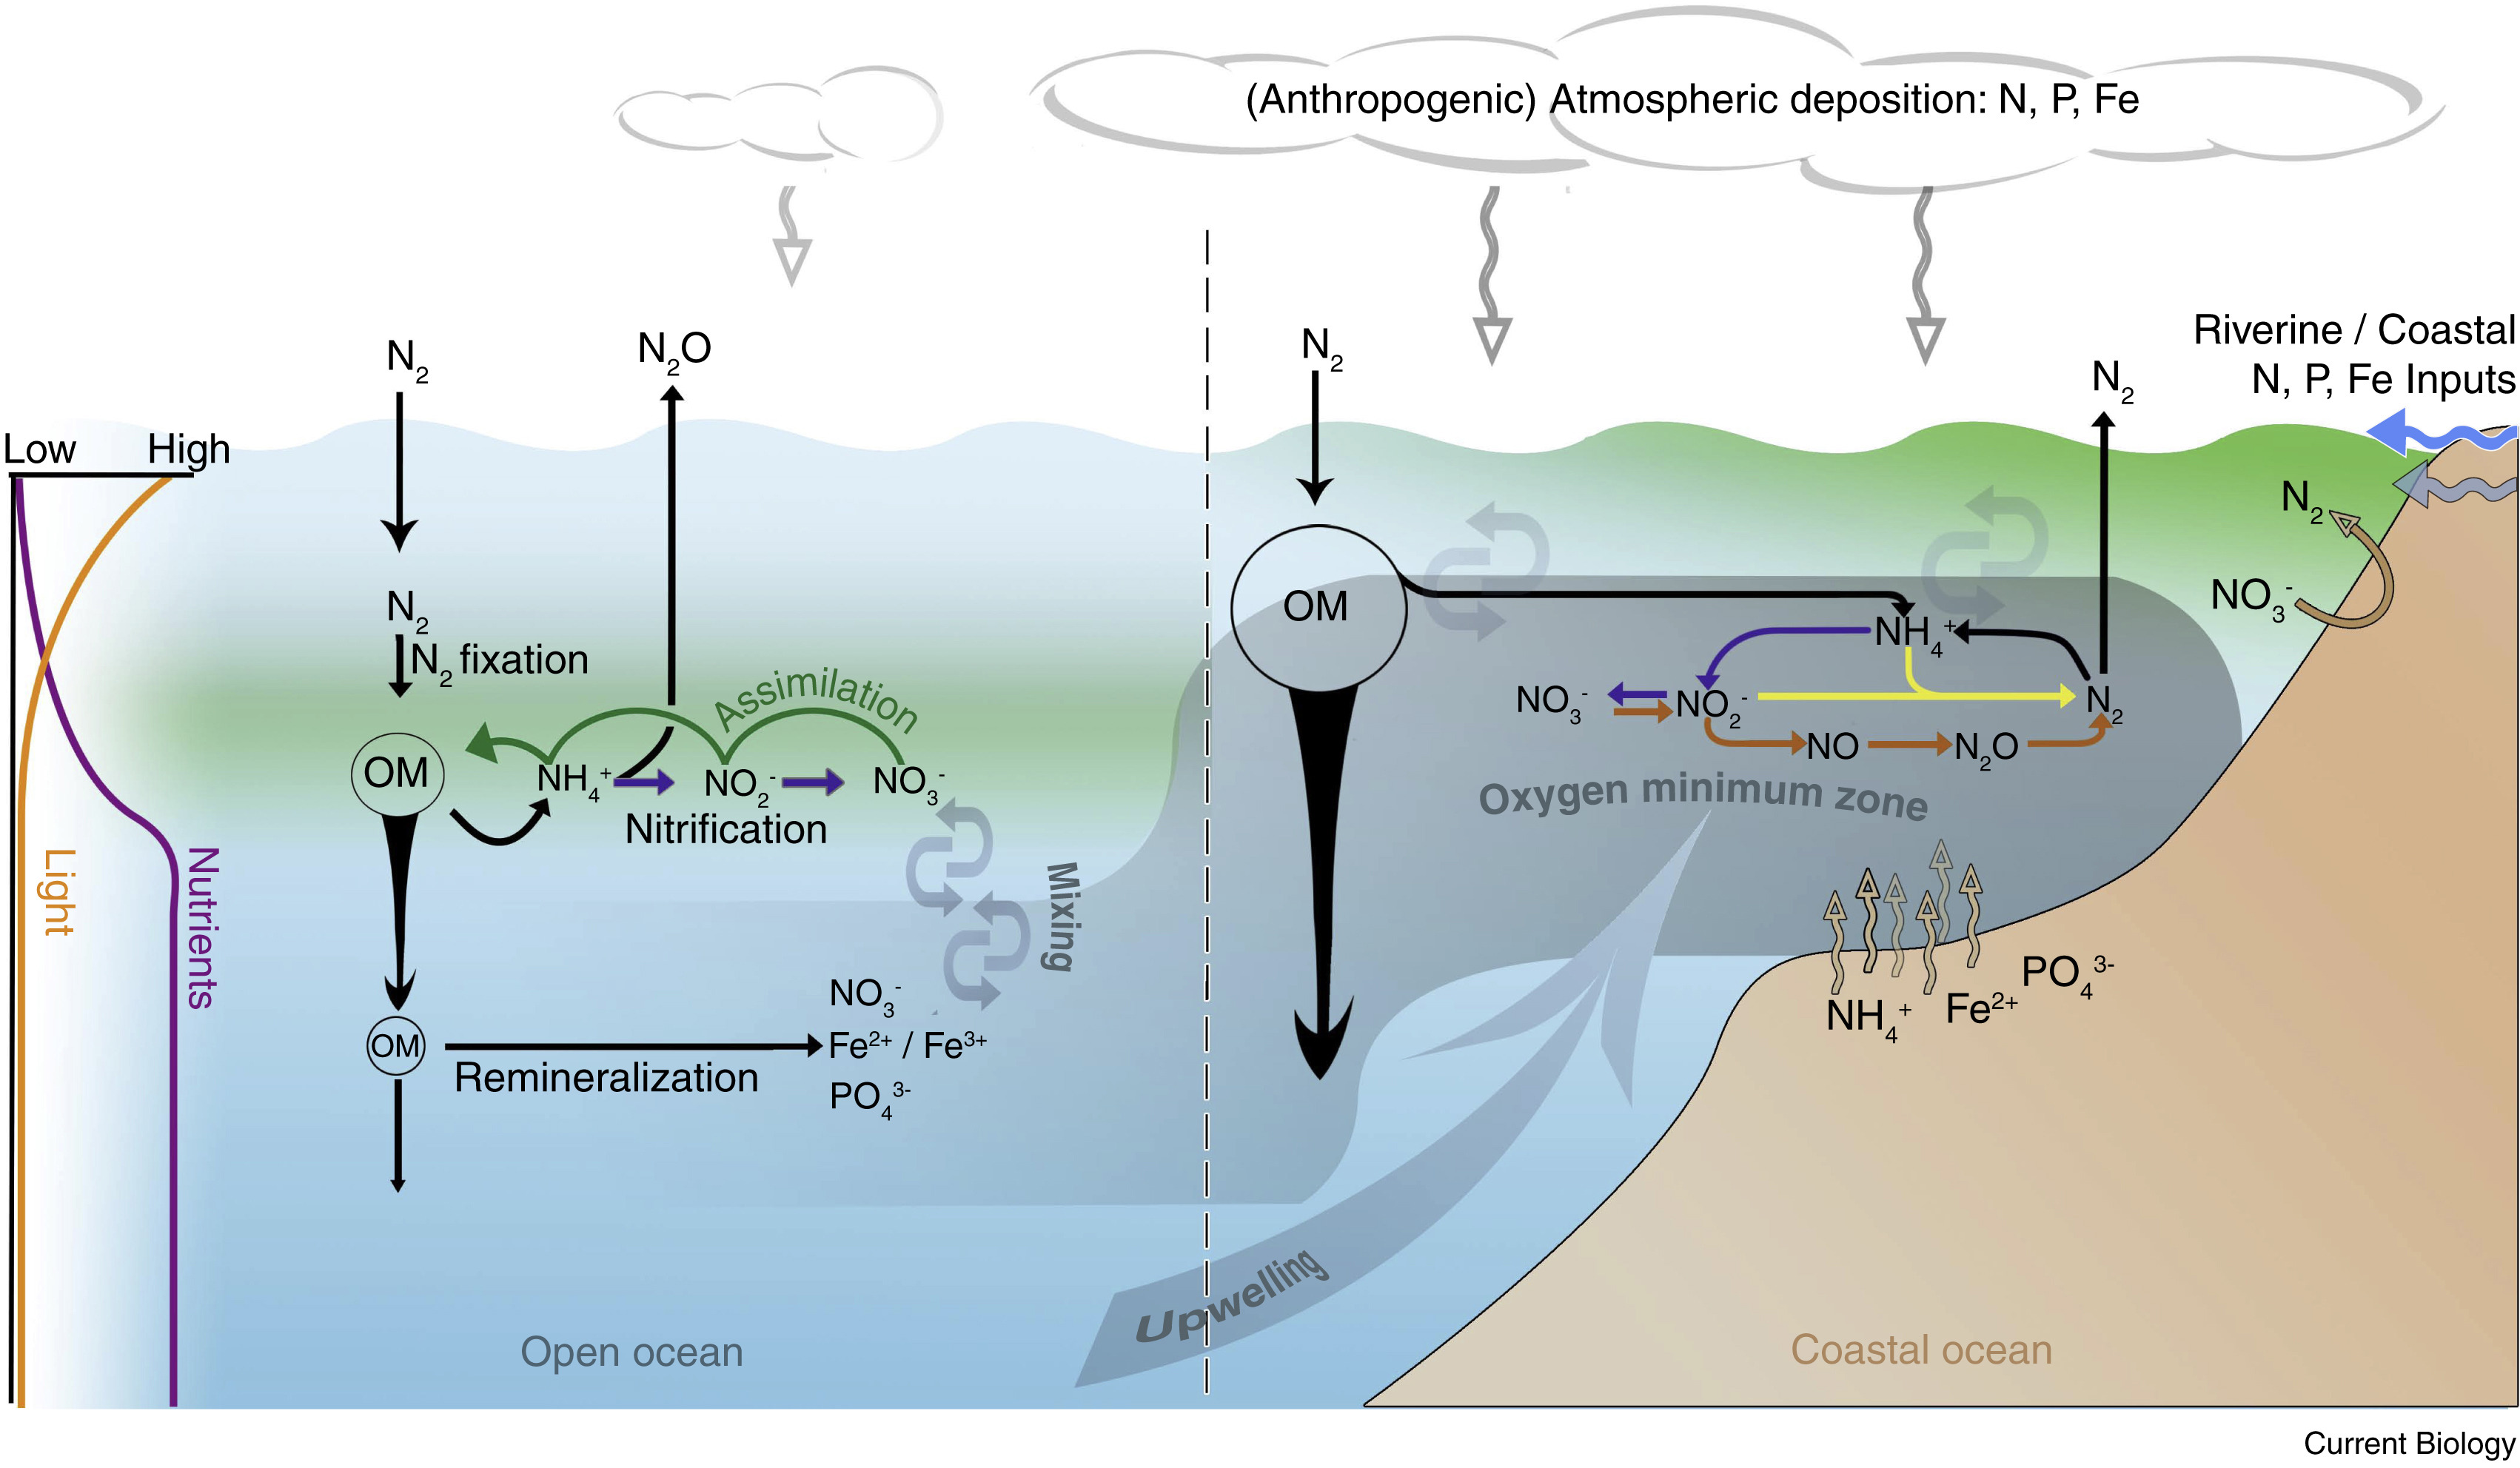
\includegraphics[width=1.0\textwidth]{figures/Chap1UpwellingFertilization.jpg}
	\centering
	\caption{Scheme of fertilization sources to the ocean as well as upwelling, riverine discharges and atmospheric deposition. The figure was taken from \cite{BrisMohr2017}.}
	\centering
	\label{Chap1UpwellingFertilization}
\end{figure}

\clearpage
\section{The northern Humboldt Current system (NHCS)}\label{Chap1NHCS}

The connection between ancient Peruvian coastal inhabitants and the sea has been apparent since pre-Columbian times \citep{Prie2014,Prie2019}. Ancient civilizations utilized the marine resources of the Peruvian coast, including a variety of fish species such as engraulids, which were dried and salted for easier transportation \citep{MarcSomm1999}. They also harvested bivalve mollusks and gastropods \citep{ChicRoja2013,WeinOsbo2022}, and macroalgae \citep{AvilPadi2020}. All of these resources flourished under the influence of the \acrfull{nhcs} and continue to generate a significant positive economic impact. Then, it is important to understand the characteristics that make this marine ecosystem unique.\\

The \acrshort{nhcs} is one of the most productive systems in the world (Fig. \ref{Chap1UpwellingSystems}), mostly located off the Peruvian coast (70\textdegree $W$ – 90\textdegree $W$; 0\textdegree $S$ – 20\textdegree $S$) and is part of the broader Peru-Chile upwelling system \citep{GradChai2018,TaraArnt2001}. \acrshort{nhcs} is considered as a highly productive marine ecosystem with a productivity of $>$ 300 $gC/cm^{2}/yr$ \citep{KampCap5}, largely due to the regular presence of upwelling-favorable winds throughout the year from 5\textdegree $S$ to 26\textdegree $S$, a feature that is rather seasonal beyond 26\textdegree $S$ \citep{BelmEche2014}. There is however seasonal and interannual variability in upwelling intensity, with intensification in the later part of the $20^{th}$ century (1960 – 2001) \citep{NaraPaul2010}.\\

\begin{figure}[ht]
	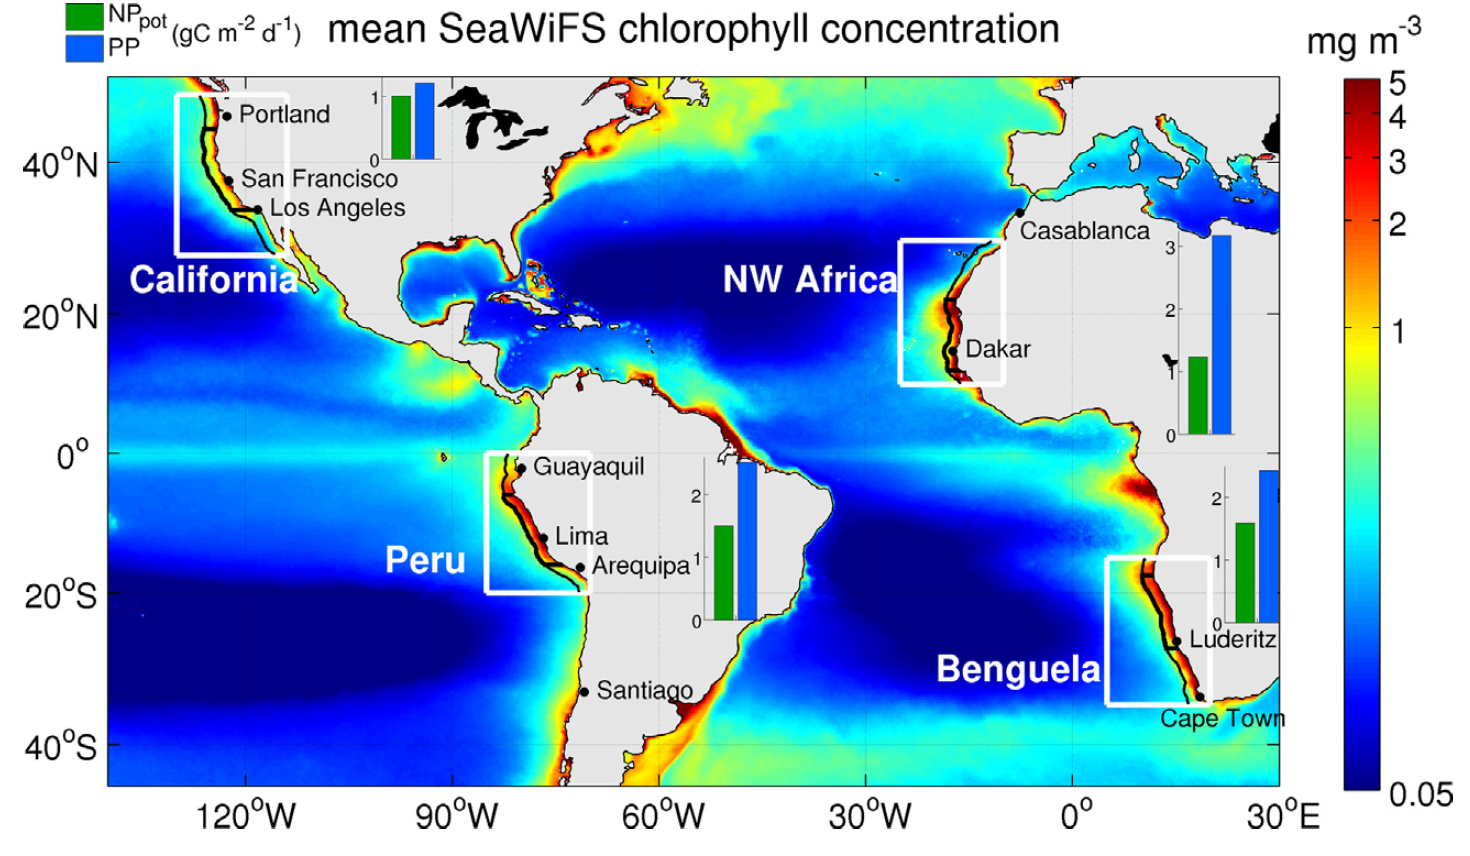
\includegraphics[width=1.0\textwidth]{figures/Chap1UpwellingSystems.png}
	\centering
	\caption{Scheme of the four most important upwelling systems represented by chlorophyll concentration measured by satellite images. The figure was taken from \cite{MessChav2015}.}
	\label{Chap1UpwellingSystems}
\end{figure}

In the \acrshort{nhcs}, water masses from different origins with specific temperature and salinity ranges converge \citep{SilvRoja2009,MontCola2010,ChaiDomi2013}. The following water masses are currently distinguished off Peru: \acrfull{tsw}; \acrfull{esw}; \acrfull{stsw}; \acrfull{essw}; \acrfull{espiw}; \acrfull{aaiw} \citep{GradChai2018}. Details of temperature and salinity range of these water masses are reported in Table \ref{TabWaterMasses} and Fig. \ref{Chap1WaterMassesNHCS}. These water masses are transported by several surface [\acrfull{epcc}; \acrfull{pcc}; \acrfull{sec}; \acrfull{poc}] and subsurface currents [\acrfull{euc}; \acrfull{pcuc}].\\

The mean circulation shows both poleward and equatorward flows (Fig. \ref{Chap1MeanCirculationNHCS}). The upper layer ($\sim$ 25 $m$) close to the coast shows a relatively strong poleward flow ($\sim$ 20 - 30 $cm/s^{-1}$) associated with the \acrshort{epcc} transporting relatively warm and fresh \acrshort{esw}. At $5$\textdegree $S$, the \acrshort{epcc} separates into two branches, one feeding the westward \acrshort{sec} and the other one continuing southward weakening until $\sim$ 8\textdegree $S$ – 9\textdegree $S$.\\

\begin{table}[ht]
\centering
\begin{tabular}{c|c|c}
\hline
\textbf{Water mass}								&
\textbf{Temperature range (\textdegree $C$)}	&
\textbf{Salinity range ($S$)}					\\
\hline
TSW				& 
23.5 - 24.5		& 
33.5 – 34.4		\\
ESW				& 
20.0 – 24.0		& 
34.6 – 35.0		\\
STSW				& 
19.0 – 23.5			& 
\textgreater{35.4}	\\
ESSW			&
8.0 – 14.0		&
34.6 – 35.0		\\
ESPIW			& 
12.0 – 14.0		& 
34.8			\\
AAIW			& 
4.0 – 7.0		& 
34.5 – 34.6		\\
\hline            
\end{tabular}
\caption{Temperature ($T$, in \textdegree $C$) and salinity ($S$) ranges of the main water-masses in the \acrshort{nhcs}. \acrfull{tsw}; \acrfull{esw}; \acrfull{stsw}; \acrfull{essw}; \acrfull{espiw}; \acrfull{aaiw}. Table modified from \cite{GradChai2018}.}
\label{TabWaterMasses}
\end{table}

Further south there is equatorward flow associated with the \acrshort{pcc} and the \acrshort{poc} transporting cold waters. The middle layer (100 – 200 $m$) is predominantly a poleward flow influenced by the \acrshort{pcuc} that extends along the entire coast, transporting \acrshort{essw} with a mean velocity that can locally reach 20 $cm/s^{-1}$. In the deeper layer (500 $m$), the average circulation is mainly equatorward transporting relatively fresh and cold \acrshort{aaiw}  \citep{ChaiDomi2013,PietTest2013}.\\

\begin{figure}[ht]
	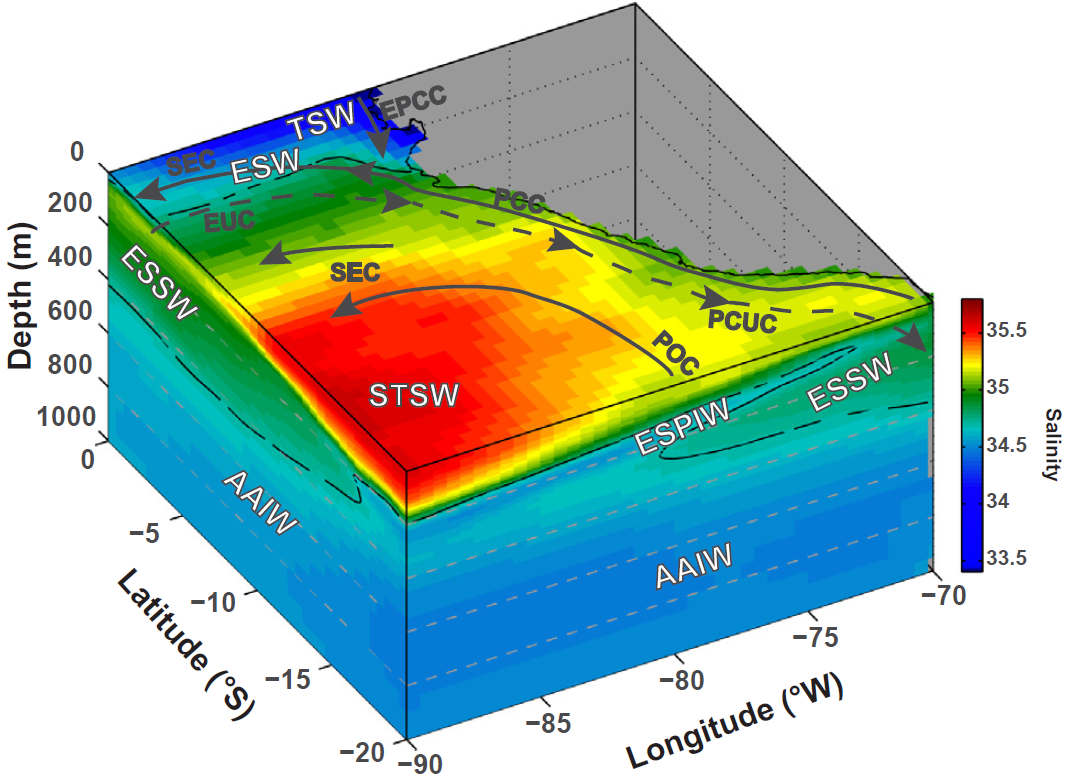
\includegraphics[width=1.0\textwidth]{figures/Chap1WaterMassesNHCS.png}
	\centering
	\caption{Main water-masses of the \acrshort{nhcs}. The color corresponds to the salinity range. The surface (thick solid lines) and subsurface (thick dashed lines) currents: \acrfull{epcc}; \acrfull{pcc}; \acrfull{sec}; \acrfull{poc}; \acrfull{euc}; \acrfull{pcuc}. Figure taken from \cite{GradChai2018}.}
	\label{Chap1WaterMassesNHCS}
\end{figure}

The mean temperature in the coastal zone off Peru is 17.6\textdegree $C$ \citep{MontPurc2003} but temperature shows strong seasonal and interannual variability, particularly due to El Ni\~{n}o events that can generate positive anomalies of more than 6\textdegree $C$  \citep{BraiMcla1987,SancCali2000,CaiBorl2014,CaiWang2017,CaiWang2018,FreuHenl2019}, and other extreme events referred to as ``coastal Ni\~{n}o" \citep{EcheCola2018,Garr2018,HuHuan2019,RodrDiaz2019,TakaMart2019}, although the above warm events could be more generally categorized as marine heatwaves, this term better describes their characteristics and physical mechanisms \citep{PietCola2021}. Along the Peruvian coast, the seasonal variability of temperature increases from north to south. This is associated with a smaller effect of upwelling in the northern zone than in the south \citep{BraiMcla1987}.\\

\begin{figure}[ht]
	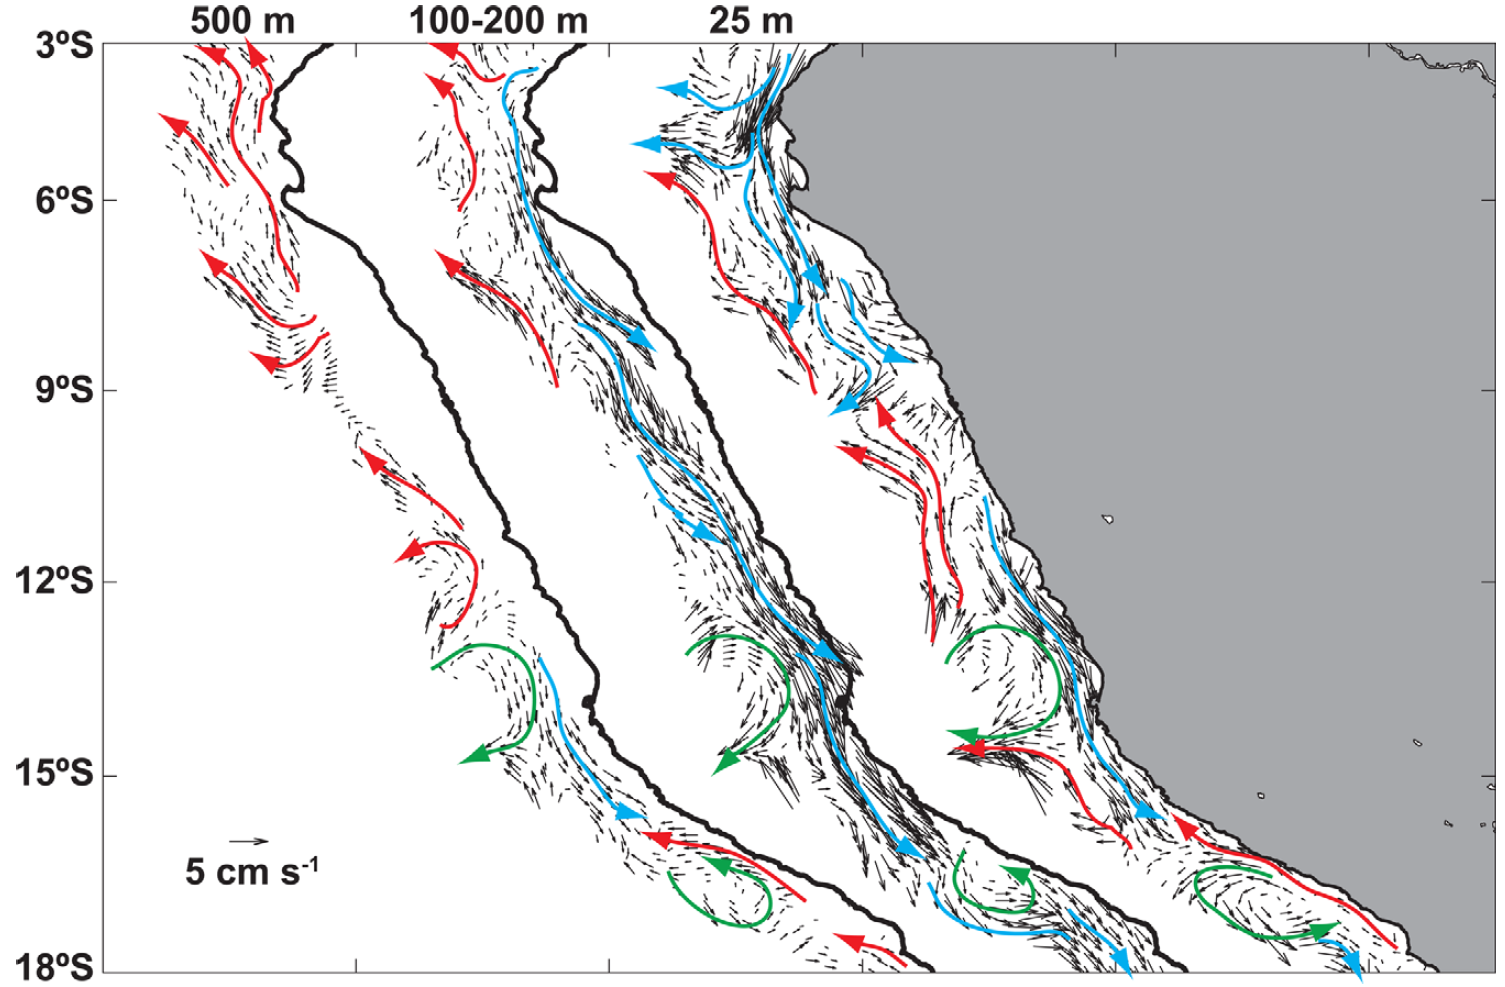
\includegraphics[width=0.8\textwidth]{figures/Chap1MeanCirculationNHCS.png}
	\centering
	\caption{Mean circulation at 25 $m$, between 100 $m$ and 200 $m$, and 500 $m$ depth. Red and blue arrows represent the equatorward and poleward flows, respectively. Green arrows indicate the presence of mesoscale cyclonic ($\sim$ 14\textdegree $S$) and anticyclonic ($\sim$ 17\textdegree $S$) eddy-like features. Figure taken from \cite{ChaiDomi2013}.}
	\label{Chap1MeanCirculationNHCS}
\end{figure}

Dissolved oxygen also shows a high spatiotemporal variability, which may at time limit the generally well oxygenated layers located near the surface \citep{EspiEche2017,EspiEche2019}. Then, \acrlong{omz} is defined as a region of the ocean exhibiting a pronounced deficiency in oxygen concentration within the water column. These zones are characterised by the presence of three distinct layers: the oxycline (upper oxygen gradient), the core (typically exhibiting oxygen concentrations below 20 $\mu M$) and the lower oxygen gradient, with eddy fluxes which contribute to the ventilation of the Peruvian oxygen minimum zone \citep{BettLope2015}. Consequently, the oxygen dynamics off the Peruvian coast can result in scenarios with a markedly low oxygen presence, which in turn reduces and limits the environment available for plankton aggregation to a depth range of 0 to 65 $m$ in the slope zone and may even be reduced to a depth range of 20 to 35 $m$ in the shelf break zone. This can result in an unusually high presence of zooplankton at the surface, which may then dissipate once the low oxygen event is overcome \citep{Judk1980}. It would appear that there is a relationship between the depth of the oxycline, macrozooplankton and forage fish (\textit{\gls{ringens}}) that can be observed at different scales, from tens of kilometers to a few hundred meters providing evidence that the submesoscale-to-mesoscale variability of the oxycline depth drives the distribution of macrozooplankton, then, shaping distribution structures of forage fish \citep{GradFabl2012,GradBert2016}.\\

Phytoplankton is consumed primarily by zooplankton, which in turn is preyed upon by small pelagic fish. These groups of organisms are subject to significant fluctuations due to seasonal and interannual (El Ni\~{n}o) physical fluctuations in oceanographic conditions. Chlorophyll, used as a proxy for primary productivity (phytoplankton), shows an annual signal, which is favored by wind stress, exhibits a seasonal maximum that shifts southward from spring to summer. This signal is in phase with the seasonal maximum in $Chl-a$ concentration detected by satellite off the coast of Chile. However, off Peru, this signal is not in phase, exhibiting seasonal maxima of $Chl-a$ in summer and the intensity of upwelling in winter \citep{EcheAumo2008,CorrHorm2012}. The spatial distributions of certain zooplankton groups exhibit a high degree of correlation with surface water masses, circulation patterns, and upwelling regions. This correlation is consistent with the ecological and dynamic partitioning of the pelagic ecosystem \citep{FernFarb2006}. However, in comparison to Peru, the signal corresponding to zooplankton is more complex, exhibiting temporal and spatial variations at different scales, with spring and summer being the most significant \citep{AronAyon2009,AronGrad2019}.\\

Thus, water masses intermingle along the coastline following the currents and constitute the biotope of one of the most productive ecosystems in the world. The \acrfull{spf} reproduce by dispersing their eggs in the surface layers, and are therefore particularly exposed to the fluctuations of this biotope which will determine in large part their chances of survival. In the following section we will describe the main species of \acrshort{spf} that inhabit this ecosystem, the Peruvian anchovy.\\

\clearpage
\section{The Peruvian anchovy (\textit{Engraulis ringens}, Jenyns 1842)}\label{Chap1PeruAnch}

Clupeoid fishes are present in pelagic environments worldwide, particularly in the productive coastal upwelling regions along the eastern margins of the Atlantic and Pacific oceans. The largest stocks are usually composed of species such as sardine, pilchard, and anchovy (\textit{Sardinops spp.} and \textit{Engraulis spp.}). The schooling behavior of clupeoids makes them easy to catch with purse seiners, resulting in some populations reaching enormous biomasses and becoming important economic resources. For example, during the early 1970s, clupeoids, particularly the Peruvian anchoveta (\textit{\gls{ringens}}), contributed approximately one-third of the world's total catches, which were around 65 million tonnes at the time \citep{ColeMcGl1998}.\\

Fig. \ref{Chap1Engraulis_ringens} shows a schematic representation of \textit{\gls{ringens}}, a \acrshort{spf}, catalogued as \textit{r}-selection species \citep{Pianka1970}, with a slightly compressed elongated body, long head, prolonged snout and very large eyes. In the dorsal part its color is dark blue, while in the ventral part it is silver \citep{Whit1988}.\\

Taxonomically, according to \acrlong{itis} (\href{https://www.itis.gov/}{ITIS}), \textit{\gls{ringens}} is located in the evolutionary tree as follows:\\

\begin{itemize}
  \centering
  \item Kingdom: Animalia
  \item Phylum: Chordata
  \item Subphylum: Vertebrata
  \item Infraphylum: Gnathostomata
  \item Superclass: Actinopterygii
  \item Class: Teleostei
  \item Order: Clupeiformes
  \item Family: Engraulidae
  \item Genus: Engraulis
  \item Species: \textit{\gls{ringens}}, Jenyns, 1842
  \item Common name: Peruvian anchovy
\end{itemize}

\begin{figure}[!]
	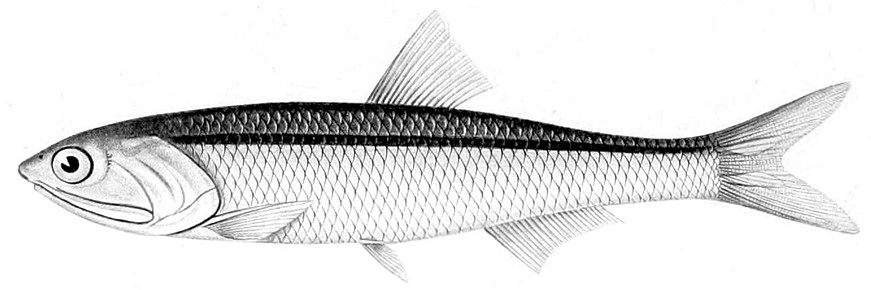
\includegraphics[width=1.0\textwidth]{figures/Chap1Engraulis_ringens.jpg}
	\centering
	\caption{Schematic representation of an adult Peruvian anchovy (\textit{\gls{ringens}}).}
	\label{Chap1Engraulis_ringens}
\end{figure}

\textit{\gls{ringens}} can reach a maximum size of 20 $cm$ and has a life span of 4 years. Its first sexual maturity may be at a size of 12 $cm$ \citep{GutiSwar2007,MarzShin2009}. This species performs external fertilization by formation of spawning aggregations, which warrants synchrony in the timing of gamete production and optimizes fertilization rates. Females release the eggs into the environment so that males can fertilize them without the need for copulation \citep{Gani2014}. During the main period of annual spawning in August-September, 16.04 \% of the female population of the central and northern anchovy stock off Peru spawned per day, this means that on average, every female spawned a new batch of eggs every 6.23 $days$ \citep{AlheAlar1984,AlheAleg1983}. In unfavorable environmental conditions, a female is capable of reabsorbing part of the ovigerous mass to obtain energy, a phenomenon known as atresia \citep{PereRoqu2008,EspiVera2009,ClarCast2012,BuitPere2018}. This species has two important spawning peaks off Peru, summer and winter, but a significant presence of eggs and larvae is reported throughout the year \citep{MarzShin2009}. Anchovy in Peru has a mainly zooplanktivorous diet, with ontogenetic and spatiotemporal variability in prey preferences, with an increase in the contribution of euphausiids to the diet as \textit{\gls{ringens}} increases in size up to 85 \% of their diet as adults (18 – 20 $cm$), in contrast, their consumption of calanoid copepods decreases with size, while diatoms make up a minimal part of their diet throughout their life span \citep{EspiBert2008,EspiBert2014}.\\

In the natural environment, eggs of \textit{\gls{ringens}} are pelagic and transparent. Their shape is ovoid, with an average major axis of 1.42 $mm$ and a minor axis of 0.71 $mm$. However, there is latitudinal variability associated with the size of the eggs, which are protected by a smooth membrane. Following hatching, the larva exhibits no pigmentation, but rather an elongated yolk sac that terminates at the posterior end of the intestine. Its body is cylindrical, with a head that is somewhat wider than the body and lacks differentiation of the mouth or jaw \citep{EinaRoja1963}. \textit{\gls{ringens}}’s early life description \citep{RiouOfel2021}, currently distinguishes 4 stages: \textbf{stage $\mathbf{1}$} from hatching to 2 \acrfull{dph} there are transparent yolk-sac larvae with closed mouth and eyes and non-pigmented body. Stage 1 ends with the opening of the mouth, pigmentation of the eyes and remnants of the yolk-sac (at length ranging from $\sim$ 2 - 4 $mm$ depending on temperature); \textbf{stage $\mathbf{2}$} from the complete absorption of the yolk sac at 3 \acrshort{dph} until larvae are between 12 - 19 \acrshort{dph} with length ranging from 8.15 - 12.97 $mm$; \textbf{stage $\mathbf{3}$} included larvae between 19-26 \acrshort{dph} and corresponding length from 10.89 - 15.03 $mm$; \textbf{stage $\mathbf{4}$}, from 33 \acrshort{dph}, larvae showed melanophores developed on the head and body, with visible gills. The first sign of schooling (continuous swimming as a group and clear evidence of active swimming behaviour, \cite{Shaw1962}) also occurred at this stage (31 \acrshort{dph}).\\

After the larval stage, anchovy juveniles already have the definitive adult form and from 12 $cm$ of length, they became available for industrial fishery \citep{MarzShin2009}. This industrial fishery is oriented almost entirely (98 \%) to indirect human consumption (feed fish) and only 2 \% is intended for direct human consumption (food fish) in canned, cured, frozen or fresh presentations \citep{FreoSuei2014}.\\

\textit{\gls{ringens}} fishery management is based on scientific monitoring of adult population indicators determined by acoustic surveys \citep{GutiSwar2007} or by the daily egg production method \citep{Ayon2000}, then allocating fishing quotas to each registered vessel and catching monitoring by technical research personnel on board these vessels \citep{KroeSanc2019}. Thus, the Peruvian anchovy has become one of the most abundant and at the same time the most studied fishery, but understanding the impact of environmental conditions on the early-life stages of anchovy and further population dynamics remains challenging.\\

\begin{figure}[!]
	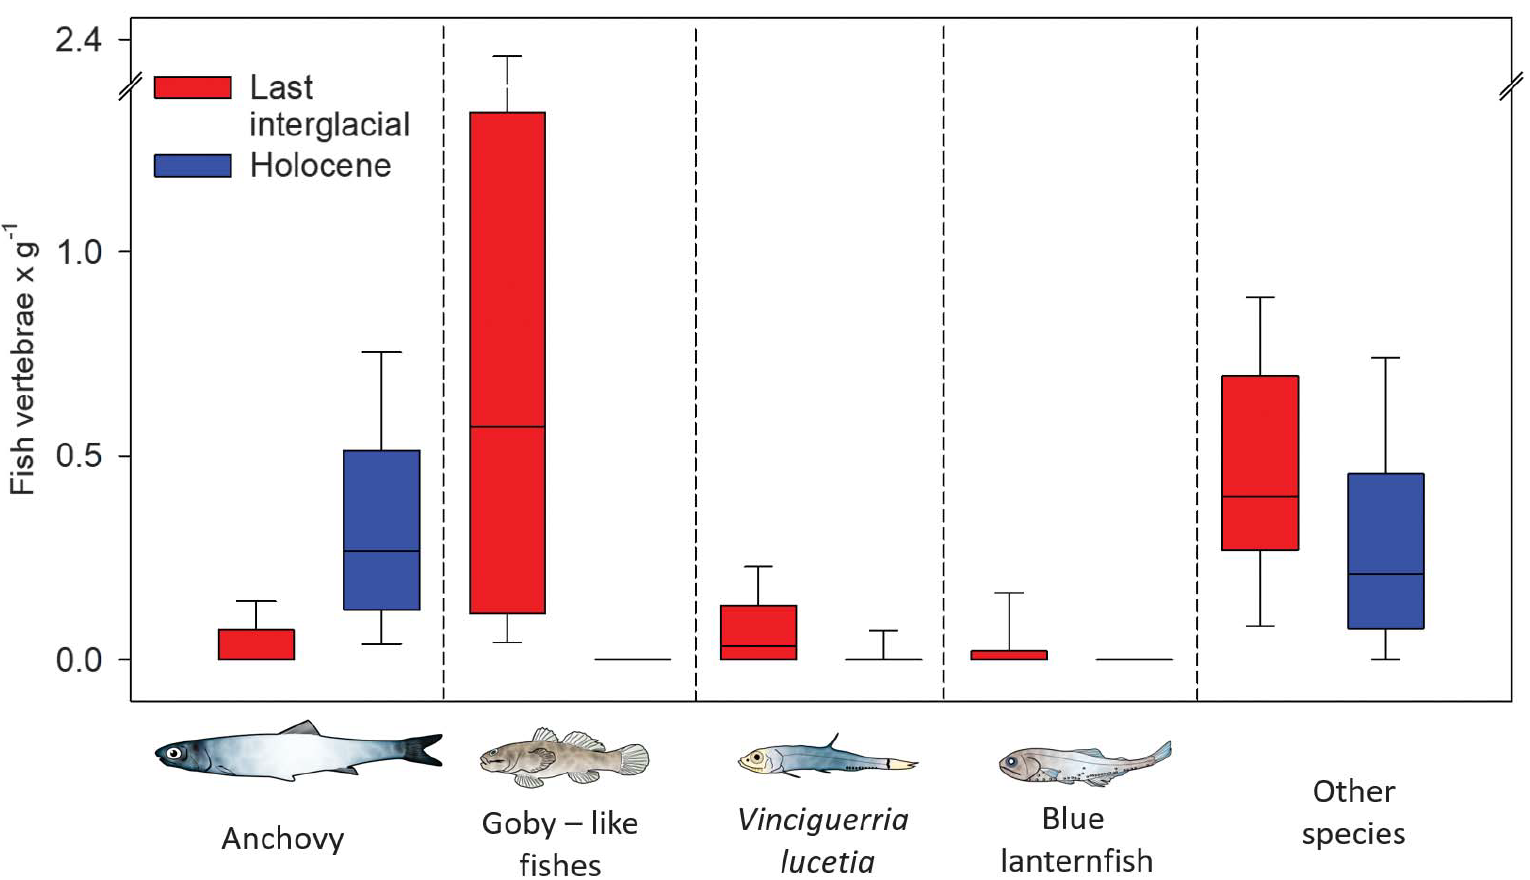
\includegraphics[width=1.0\textwidth]{figures/Chap1VertebraeAbundances.png}
	\centering
	\caption{Fish vertebrae abundances during the last interglacial and Holocene. Figure taken from \cite{SalvSchn2022}.}
	\label{Chap1VertebraeAbundances}
\end{figure}

However, this abundance has not been constant at geological scales as shown by palaeoceanographic records, which have evidenced that \textit{\gls{ringens}} has populated the \acrshort{nhcs} for thousands of years under a naturally varying climate with high variability during the last 25 $ky$ \citep{SalvField2018,SalvGuti2019,SalvSchn2022}, playing an important role transferring energy from lower to higher levels of the food web \citep{ChecAsch2017}. Fig. \ref{Chap1VertebraeAbundances} show we are currently in the Holocene period, characterized by a great abundance of the Peruvian anchovy biomass, however, during the last interglacial period, with warm and oxygen-poor environmental conditions, the presence of \textit{\gls{ringens}} was considerably lower, and that conditions favored the flourishing of other mesopelagic fishes \citep{SalvSchn2022}, environmental conditions that could be repeated in a climate change scenario \citep{EcheGeva2020}.\\

Thus, environmental variability in a complex system such as the \acrshort{nhcs} and its impact on \textit{\gls{ringens}} abundance has been extensively studied under different approaches, one of them being modelling.\\

\clearpage
\section{Modelling studies on \textit{E. ringens}}\label{Chap1ModeAnch}

The inherent impossibility of monitoring the entire ecosystem at high frequency and resolution is a major limitation of ichthyoplankton in situ observations. This is where models, become relevant, allowing us to integrate multiple spatio-temporal scales and to testing hypotheses on ichthyoplankton dynamics in response to the different  environmental forcing’s, including forecasting scenarios \citep{GearDode2020}.\\

Despite many modelling studies conducted in the past \citep{LettPenv2007,BrocLett2008,GutiRami2008,OlivPena2011,XuChai2013} that have tried to explain a relationship between environmental variability and the success of anchovy recruitment, much remains to be understood due to the high plasticity of this species and its adaptation capacity to environmental changes \citep{EspiBert2008,EspiBert2014,CanaAdas2018,PlazCern2018}.\\

Early modelling studies for the understanding of \acrshort{nhcs} dynamics were done by hydrodynamic modelling reproducing general ocean circulation patterns \citep{PenvEche2005,ColaMcwi2012}, its interannual variability \citep{ColaCape2008,EspiEche2017}, its potential changes under future climate scenarios \citep{OerdCola2015,EcheGeva2020}. These previous works provide us a strong physical basis for ecological studies in the \acrshort{nhcs}.\\

From a realistic representation of the physical environment, researchers have tested \cite{Baku1998} triad hypothesis for \acrshort{spf} recruitment and early life stages survival by quantification of enrichment, concentration and retention processes in \acrshort{nhcs} \citep{LettPenv2007} and complementarily also in the Benguela upwelling ecosystem \citep{LettRoy2006}, in both cases, the coastal zone emerged as the most favorable by analyzing the spatial distribution and seasonal variability of these indices. Further modelling studies showed that \textit{\gls{ringens}} larval retention patterns displayed strong seasonal variability possibly modulated by vertical distribution of individuals in regards to the vertical current structure, resulting in a maximal coastal retention close to the surface in winter and in deeper layers in summer. Also, a partial match between dates and locations of enhanced retention and observed egg concentration patterns was found \citep{BrocLett2008}. Additionally, in the region of Chile where the same species also thrives, a study was conducted to examine the transport of eggs and larvae from spawning zones in central Chile to historical nursery areas. The results indicated that the highest pre-recruitment values were mainly found in winter \citep{ParaCola2012}.\\

In the four main \acrfull{ebus}, the reproductive strategy of \acrshort{spf} species, dominated by anchovies and sardines, is a trade-off between larval retention and larval food availability. In the \acrshort{nhcs}, the winter spawning benefit both from high zooplankton and shelf retention rates, which may explain the particularly  large \acrshort{spf} populations \citep{BrocCola2009,BrocLett2011}. Climate change might negatively impact \textit{\gls{ringens}} recruitment due to a reduction in the size of the habitat due to a reduction in ecosystem productivity not compensated by increased retention rates \citep{BrocEche2013}. The effects of temperature and food availability on larval growth could modulate this result; as it was suggested that \acrfull{enso} events may negatively impact \textit{\gls{ringens}}  recruitment by reducing the larval growth speed due to changes in food availability \citep{XuChai2013,XuRose2015}. The seasonal variability in larval growth speed was not explicitly taken into account in previous studies, a gap that was addressed in the present work.\\

In order to investigate the impact of environmental variability on early life stages of \acrshort{spf}, we developed \gls{ich-deb}, an individual-based model \citep{LettVerl2008} including larval retention processes and a \acrfull{deb} \citep{Kooi2009} bioenergetic module for larval growth. Using this tool, we assessed the effect of hydrodynamic simulations horizontal resolution on simulated larval retention patterns in chapter \ref{Chap2}, then, we studied the impact of the biological processes on simulated larval growth and recruitment and the effect of the upper thermal limit in chapter \ref{Chap3}, for which lab experiments are lacking. Finally in chapter \ref{Chap4} and \ref{Chap5}, we presented a complete life cycle growth model of the Peruvian anchovy with potential uses for the study of juvenile and adult behaviour.\\

\clearpage

%\section{The recruitment problem}\label{Chap1RecruProb}
%Fish populations can vary greatly over time, from interannual to millennial fluctuations. For short-lived fish, these two scales of variability are comparable in magnitude, indicating that reproductive success and recruitment are the main factors contributing to abundance. Reproductive success refers to the number of offspring an individual produces per breeding event or over their lifetime, which is closely related to the environment in which the parents develop and is something that can be monitored through research cruises during the spawning season, and in the other hand to address the ``recruitment problem'', which is the lack of knowledge to explain recruitment variability, a solid theoretical basis and practical methods are necessary, however, monitoring early life stages in the natural environment is inherently difficult, posing a great challenge with more questions than answers.
%
%Theories on how environmental conditions affect recruitment success, based on the survival/mortality of early life-history stages, can be categorized into mechanistic and synthesis theories. Mechanistic theories focus on particular physical processes, while synthesis theories aim to integrate the various mechanistic processes into a single conceptual framework. Although some theories have been successfully tested, there has been little success in reliably predicting recruitment success based on environmental conditions \citep{ColeMcGl1998}.
%\clearpage
